\documentclass[12pt]{article}
\usepackage{amsmath}
\usepackage{amssymb}
\usepackage[table]{xcolor}
\usepackage{tikz}
\usepackage[margin=1in]{geometry}
\usepackage{framed}
\usepackage{tabularray}
\usepackage{graphicx}
\usepackage[colorlinks=true, linkcolor=blue, bookmarks=true, bookmarksopen=true]{hyperref}
\usepackage{float}
\usepackage{enumitem}
\usepackage{svg}
\usepackage{caption}
\UseTblrLibrary{varwidth}

\newlength{\tablelinewidth}
\setlength{\tablelinewidth}{0.75pt}
\setlength{\arrayrulewidth}{\tablelinewidth}
\usetikzlibrary{decorations.pathmorphing, shapes.geometric, calc}

\title{Module 1: Introduction to Machine Learning}
\begin{document}
\maketitle
\linespread{1.5}

\section{Fundamentals of Machine Learning}
Machine learning is a type of artificial intelligence (AI) that allows machines to learn without being explicitly programmed. A more formal "well-posed" definition of "learning" is:

\begin{framed}
  A computer program is said to learning from experience (E) with respect to some task (T) and some performance measure (P) if its performance at task T, as measured by P, improves with experience E.
\end{framed}

The core process consists of:
\begin{itemize}
  \item \textbf{Data Storage}: retrieval of raw data.
  \item \textbf{Abstraction}: extracting knowledge and training models.
  \item \textbf{Generalization}: applying knowledge to new similar tasks.
  \item \textbf{Evaluation}: measuring the utility of the learned knowledge.
\end{itemize}

\subsection{Applications}
\begin{itemize}
  \item \textbf{Retail/Finance}: Consumer behavior analysis, fraud detection, and stock market forecasting.
  \item \textbf{Manufacturing/Telecommunications}: System optimization, troubleshooting, and network quality of service.
  \item \textbf{Medicine}: medical diagnosis.
  \item \textbf{Telecommunications}: Call patterns are analyzed for network optimization and maximizing the quality of service.
  \item Large amounts of data in physics, astronomy, and biology can only be analyzed fast enough by computers.
\end{itemize}

\subsection{Terms}
\begin{itemize}
  \item \textbf{Abstraction}: Process of extracting knowledge about stored data. This involves creating general concepts about the data as a whole. The creation of knowledge involves application of known models and creation of new models.
  \item \textbf{Training}:  process of fitting a model to a dataset. When the model has been trained, the data is transformed into an abstract form that summarizes the original information.
  \item \textbf{Generalization}: The process of turning the knowledge about stored data into a form that can be utilized for future action. The goal is to discover those properties of the data that will be most relevant to future tasks.
  \item \textbf{Evaluation}: process of giving feedback to the user to measure the utility of the learned knowledge. This feedback is then utilised to effect improvements in the whole learning process
  \item \textbf{Inductive bias}: set of necessary assumptions an algorithm uses to predict outputs for inputs it has never encountered before. (eg: in linear regression, model assumes that data has some linear pattern)
\end{itemize}

\subsection{Types of Machine Learning}
\begin{enumerate}
  \item \textbf{Supervised Learning}: Algorithms are trained on labeled data where both the input and desired output are known. Subclasses:
    \begin{itemize}
      \item \textbf{Classification}: Predicting discrete output values (e.g., identifying "Spam" or "Not Spam").
      \item \textbf{Regression}: Predicting continuous real-number output values (e.g., house prices based on square footage).
    \end{itemize}
  \item \textbf{Unsupervised Learning}: Algorithms analyze unlabeled data to discover hidden patterns. Subclasses:
    \begin{itemize}
      \item \textbf{Clustering}: ouping similar data points together (e.g., segmenting customers).
      \item \textbf{Association}: Handing relationships between variables (e.g., products bought together).
    \end{itemize}
  \item \textbf{Reinforcement Learning}: An agent learns to maximize rewards through trial and error by taking actions within an environment.
\end{enumerate}

\section{Construction of Model}
Constructing a machine learning model is a systematic process of transforming raw experience into a generalized mathematical representation. The workflow typically follows 7 stages:

\subsection{Problem Definition (Defining Task T)}

Before gathering data, the objective must be clearly defined. This involves identifying the type of learning required:

\begin{itemize}
  \item \textbf{Supervised}: Mapping inputs to known labels (Classification) or continuous values (Regression).
  \item \textbf{Unsupervised}: Discovering hidden structures or clusters in unlabeled data.
  \item \textbf{Reinforcement}: Learning optimal actions through trial-and-error within an environment to maximize rewards.
\end{itemize}

\subsection{Data Acquisition and Storage}

This stage focuses on gathering "Experience (E)". Data is retrieved from various sources—such as sensors, databases, or logs—and stored in a format accessible for computation. The quality and quantity of data at this stage directly determine the potential ceiling of the model's performance.

\subsection{Data Preprocessing and Abstraction}

Raw data is often noisy or incomplete. In this stage raw data is converted into a form suitable for learning. This involves:
\begin{enumerate}
  \item \textbf{Data Cleaning}: Handling missing values, removing outliers, and resolving inconsistencies.
  \item \textbf{Normalization}: Scaling numerical features to a uniform range (e.g., 0 to 1) to ensure that features with larger magnitudes do not disproportionately influence the model.
  \item \textbf{Feature Engineering}: Selecting the most relevant variables (Feature Selection) or transforming high-dimensional data into a more efficient representation (Feature Extraction) using techniques like Principal Component Analysis (PCA).
\end{enumerate}

\subsection{Model Selection}

Choosing an algorithm means identifying the nature of data, and then select model with appropriate \textbf{Inductive Bias}. For example, choosing a Linear Regression model assumes the relationship is a straight line, while choosing a Neural Network assumes the relationship can be modeled as a complex composition of non-linear functions.

\subsection{Training and Optimization}

During training, the algorithm adjusts its internal parameters (such as weights and biases) to minimize the error between its predictions and the actual data.

The data is split into 3 sets:
\begin{enumerate}
  \item \textbf{Training set}: For training the model. It is usually 70-80\% of dataset is used for training
  \item \textbf{Validation set}: For estimating the model's fit while tuning it's parameters and preventing overfitting. After been used once, the validation set effectively becomes part of training data.
  \item \textbf{Test set (publication set)}: For providing an unbiased final evaluation of a trained model's performance on unseen data. This is used for others to test the model. It typically 10-30\% of whole dataset.
\end{enumerate}

\begin{enumerate}
  \item \textbf{Optimization}: In models like Multi-Layer Perceptrons, this is often done via \textit{Backpropagation}, where the gradient of the loss function is calculated and used to update weights in reverse order from the output layer to the input layer.
  \item \textbf{Iteration}: The model repeatedly processes the training data until the performance converges or reaches a satisfactory level.
\end{enumerate}

\subsubsection{Underfitting (High Bias)}
Underfitting occurs when a model is too simple to capture the underlying trend of the data. It makes strong, often incorrect assumptions about the dataset. It performs poorly on the training data and poorly on the test data.

\subsubsection{Overfitting (High Variance)}
Overfitting occurs when a model is overly complex and begins to "memorize" the training data, including its random noise and outliers, rather than learning the general pattern. It shows near-perfect accuracy on training data but fails significantly on unseen test data.

\subsubsection{Triple Trade-off}
There is a unavoidable trade off between three variables
\begin{enumerate}
  \item The size or complexity of the learned model
  \item The amount of training data
  \item The generalization error on new examples
\end{enumerate}

\subsection{Evaluation (Performance Measure P)}

Once trained, the model's utility must be measured. It is critical to use a separate "Test Set" that the model has never seen during training to check for **Generalization**.
\begin{enumerate}
  \item \textbf{Metrics}: Depending on the task, performance is measured using metrics like **Precision, Recall, F1-Score**, or **ROC curves**.
  \item \textbf{Resampling}: Techniques like **K-Fold Cross-Validation** are used to ensure the performance is robust and not a result of a specific, lucky split of the data.
\end{enumerate}
\subsection{Deployment and Generalization}

The final stage is the application of the model to real-world tasks. A successful model demonstrates high generalization, meaning it maintains its predictive accuracy when processing entirely new data points. Continuous monitoring is often required to ensure the model does not "drift" as real-world data patterns evolve over time.

\section{Some Other concepts}
\subsection{Hypothesis}
Hypothesis ($h$) is a single mathematical function that an algorithm "proposes" as the solution to a learning task. It represents a specific mapping from the input features ($X$) to the predicted output ($Y$).
\subsubsection{\texorpdfstring{Hypothesis Space ($\mathcal{H}$)}{Hypothesis Space (H)}}
It is complete set of all possible functions that the learning algorithm is capable of considering. It is essentially the "search space" or the set of candidate solutions defined by the algorithm's architecture.

\subsubsection{\texorpdfstring{Version space ($V$)}{Version space (V)}}
It is subset of hypothesis space ($\mathcal{H}$) that are consistent with the observed training data ($D$).

\subsubsection{Consistency}
A specific hypothesis ($h$) is consistent with the training data ($D$) if and only if it produces a correct output for every single example in the training set.
$$h(x) = c(x) \text{ for all examples }(x, c(x)) \text{in the training data}$$

\subsubsection{Most General hypothesis (G)}
Hypothesis that makes no restrictions at all, and specifically there exists no other hypothesis $h$ that is more general than $G$. It can be said that:
$$\nexists h : G <_g h$$
In algorithms like \href{https://www.geeksforgeeks.org/machine-learning/ml-candidate-elimination-algorithm/}{Candidate Elimination}, the algorithm classifies every potential instance as a "Positive" example, regardless of its features and then incrementally shrinks the version space only when it encounters negative examples that it must exclude.

\subsubsection{\texorpdfstring{Most Specific hypothesis (\boldmath$S_0$)}{Most Specific hypothesis (S0)}}
Hypothesis that makes the most restrictive assumptions possible. In other words, there exists no other hypothesis $h$ that is more specific than $S_0$:
$$\nexists h : S_0 >_g h$$

In training algorithms like \href{https://www.geeksforgeeks.org/machine-learning/ml-find-s-algorithm/}{Find-S}, initially, the algorithm classifies every potential instance as a "Negative" example. During the training process, the model gradually generalizes its version space it only as much as necessary to cover observed positive training examples.
\begin{center}
  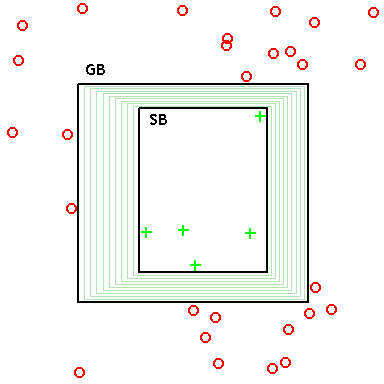
\includegraphics[width=.3\linewidth]{hyp.png}
\end{center}

\vspace*{1cm}
The goal of learning is to find a hypothesis that sits between these two boundaries, covering all positive examples without including any negative ones

\subsection*{Problem}
\textbf{Example: Is the fruit Sweet?}

\begin{table*}[ht]
  \centering
  \begin{tabular}{lll}
    Fruit & color  & sweet \\
    \hline
    F1    & Red    &  Y    \\
    F2    & Green  &  N    \\
    F3    & Yellow &  Y
  \end{tabular}
  \caption*{Training data}
\end{table*}

1. List entire hypothesis space (Possible rules)
\begin{itemize}
  \item $h1$ : sweet if color= red
  \item $h2$ : sweet if color= green
  \item $h3$ : sweet if color= yellow
  \item $h4$ : sweet if color= red or yellow
  \item $h5$ : sweet if color= red or green
  \item $h6$ : sweet if color= green or Yellow
  \item $h7$ : sweet if color= red or green or yellow ( any color)
  \item $h8$ : nothing is sweet
\end{itemize}

2. Eliminate inconsistent Hypothesis
From the training data:
Red- Y

Green- N

Yellow- Y

Remove hypothesis that:

Predict green is sweet : h2, h5, h6, h7

Miss Red or Yellow: h1, h3, h8

3. Final version space (VS)
Version space $VS_H$ Only consistent hypothesis:

\textbf{\boldmath$h4$: sweet if color is Red or Yellow}

\section{Vapnik- Chervonenkis (VC) Dimension}
\begin{framed}
  The VC dimension of H, denoted as $VC(\mathcal H)$, is the maximum cardinality (size) of a set of points that can be shattered by $\mathcal H$.
\end{framed}
ie. It is the capacity of a classification algorithm, and is defined as the \textbf{maximum cardinality of the points that the algorithm is able to shatter}.
VC dimension is a measure of the capacity or complexity of a space of functions that can be learned by a classification algorithm.

\subsubsection*{Shattering}
A set of points $S$ is said to be shattered by a hypothesis space $\mathcal H$ if, for every possible labeling of those points, there exists a hypothesis $h$ in $\mathcal H$ that classifies them perfectly.
For $N$ points, there are $2^N$ possible ways to label them (e.g., as positive or negative). If the model can realize all $2^N$ configurations, it shatters the set.

\section{Supervised Learning}
Supervised learning is a category of machine learning where an algorithm is trained on a labeled dataset. This means that for every input provided during the training phase, the corresponding correct output (or "ground truth") is already known. The goal is to learn a mapping function $f(x)$ such that when presented with new, unseen input data ($x$), the model can accurately predict the output ($Y$). Mathematically, this is expressed as $Y=f(x)$. There are two class of SL algorithms: Regression analysis, Classification.

\subsection{Regression analysis}
Regression analysis is a method for estimating the relationship between a dependent variable $Y$ (called the outcome) and one or more independent variables $X$ (called regressors, predictors or features). Regression models are used to forecast outcomes based on the predictors. Mathematically represented as:
$$Y_i = f(X) + \epsilon$$
Where $\epsilon$ is some noise which are not directly observed in the data.

\subsubsection*{Types of regression models}
\begin{itemize}
  \item \textbf{Linear Regression}: Here the model specification is that the dependent variable, $y_i$ is a linear combination of the parameters. The output is thus can be modeled as a linear equation of the form:
    $$Y = \sum_i \beta_i x_i$$
    This will reduce to a line in 2-D (called simple linear regression), a plane in 3D or hyperplane in higher dimensions (multiple linear regression).

    \begin{figure*}
		\centering
      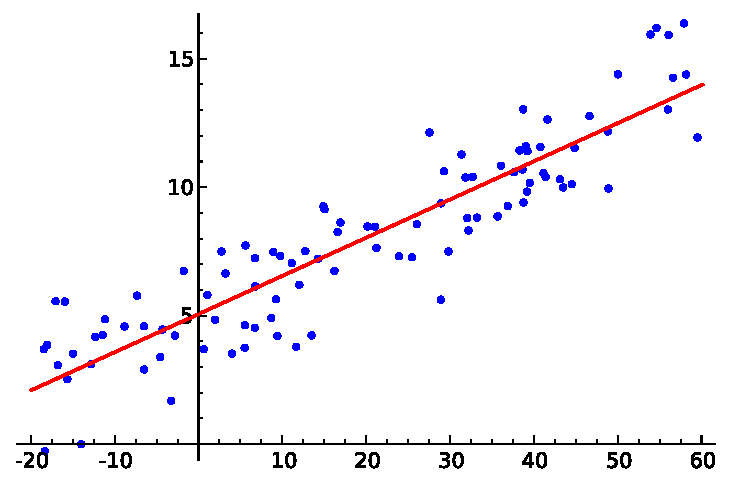
\includegraphics[width=.4\linewidth]{Linear_regression.pdf}
      \caption*{Linear regression}
    \end{figure*}

  \item \textbf{Polynomial Regression}: It models the relationship as an $n^\textrm{th}$ degree polynomial. This is essentially linear regression where the features are transformed into higher powers
  $$Y = \sum_i \alpha_i x^i$$
  \item \textbf{Logistic Regression}: It used when dependent variable is of binary nature (1/0, True/false). Here a probability function is determined whose output is between 0 and 1.
\end{itemize}

\subsubsection{Linear Regression}


\section{Unsupervised Learning}

\section{Supervised vs Unsupervised}
\begin{tblr}{
    row{1} = {bg=azure3, fg=white, font=\centering\bfseries},
    hlines, vlines, width=\linewidth, colspec = {X[m]X[m]X[m]},
    measure = vbox, stretch = -1, rowsep = 4pt
  }
  Parameters & Supervised & Unsupervised \\
  Input data &  Algorithms are trained using labeled data & Algorithms are used against data that is not labeled \\
  Computational Complexity & Simpler method & Computationally complex \\
  Accuracy & Highly accurate & Less accurate \\
  No. of classes & No. of classes is known & No. of classes is not known \\
  Data analysis & Uses offline analysis & Uses real-time analysis of data \\
  Algorithms used & {
    \begin{itemize}[nosep, leftmargin=*]
      \item Linear, Logistic Regression
      \item random forest
      \item Support Vector machine
      \item Neural networks
    \end{itemize}
  } &
  {
    \begin{itemize}[nosep, leftmargin=*]
      \item K-Means Clustering
      \item Hierarchical Clustering
      \item Apriori algorithm, etc.
    \end{itemize}
  }
\end{tblr}

\section{Reinforcement Learning}

\section{Bayesian Theory and Classifier}
\begin{itemize}
  \item \textbf{Bayes Theorem}: A mathematical principle describing how to update probabilities given additional information. Mathematically represented as $P(A|B) = \frac{P(B|A) \cdot P(A)}{P(B)}$.
  \item \textbf{Naive Bayes}: assifier A simplified multiclass classifier that assumes all features are independent (no dependency between feature 1 and feature 2) and that the class has conditional independence.
\end{itemize}

\section{Building a Machine Learning Model}
The typical workflow involves several critical stages:
\begin{enumerate}
  \item \textbf{Problem Definition} Clearly defining what the model should predict.
  \item \textbf{Data Collection/Preparation} Gathering, cleaning (handling missing values), and splitting data into training and test sets.
  \item \textbf{Algorithm Selection} Choosing the appropriate model (e.g., Decision Tree vs. Neural Network) based on the problem type.
  \item \textbf{Training} Feeding the training data into the algorithm to minimize error using optimization techniques like gradient descent.
  \item \textbf{Evaluation} Testing the model on unseen data to ensure generalization.
\end{enumerate}
\end{document}
